% XeLaTeX

\documentclass[a4paper,10pt]{article}

\usepackage[T1]{fontenc}

\usepackage[british]{babel}
\usepackage{bookmark}
\usepackage{color}
\usepackage[babel=true]{csquotes}
\usepackage{datetime}
   \newdateformat{monthyeardate}{\monthname[\THEMONTH] \THEYEAR}
\usepackage{fontspec}
\usepackage{graphicx}
\usepackage{hyperref}
   \definecolor{lcolor}{rgb}{0,0,0}
   \hypersetup{colorlinks,breaklinks,urlcolor=lcolor,linkcolor=lcolor}
\usepackage[big]{layaureo}
\usepackage{longtable}
\usepackage{marvosym}
\usepackage{multirow}
\usepackage{parskip}
\usepackage{supertabular}
\usepackage{titlesec}
\usepackage{url}
\usepackage[usenames,dvipsnames]{xcolor}
\usepackage{xltxtra}
\usepackage{xunicode}

\newenvironment{literature}{%
   \parskip6pt\parindent0pt\raggedright
   \def\lititem{\hangindent=1cm\hangafter1}}{%
   \par\ignorespaces}

\defaultfontfeatures{Mapping=tex-text}
\setmainfont[SmallCapsFont=fontin_small_caps.otf,BoldFont=fontin_bold.otf,ItalicFont=fontin_italic.otf]{fontin.otf}

\titleformat{\section}{\Large\scshape\raggedright}{}{0em}{}[\titlerule]
\titlespacing{\section}{0pt}{15pt}{15pt}

\setlength{\fboxsep}{0pt}
\setlength{\fboxrule}{2pt}

\begin{document}

\pagestyle{plain}
\pagenumbering{Roman}
\font\fb=''[cmr10]''

\par{\centering
   {\Large\textsc{Dr\hspace{0.5pt}. phil\hspace{0.5pt}.}
   }\bigskip\par}

\par{\centering
   {\Huge\textsc{Alexander Max Bauer}
   }\bigskip\par}

\vspace{1cm}
\par{\centering
   {\Large\textsc{Curriculum Vitae}
   }\bigskip\par}

\par{\centering
   {\Large\textsc{\monthyeardate\today}
   }\bigskip\par}

\vfill
\begin{center}
   \fbox{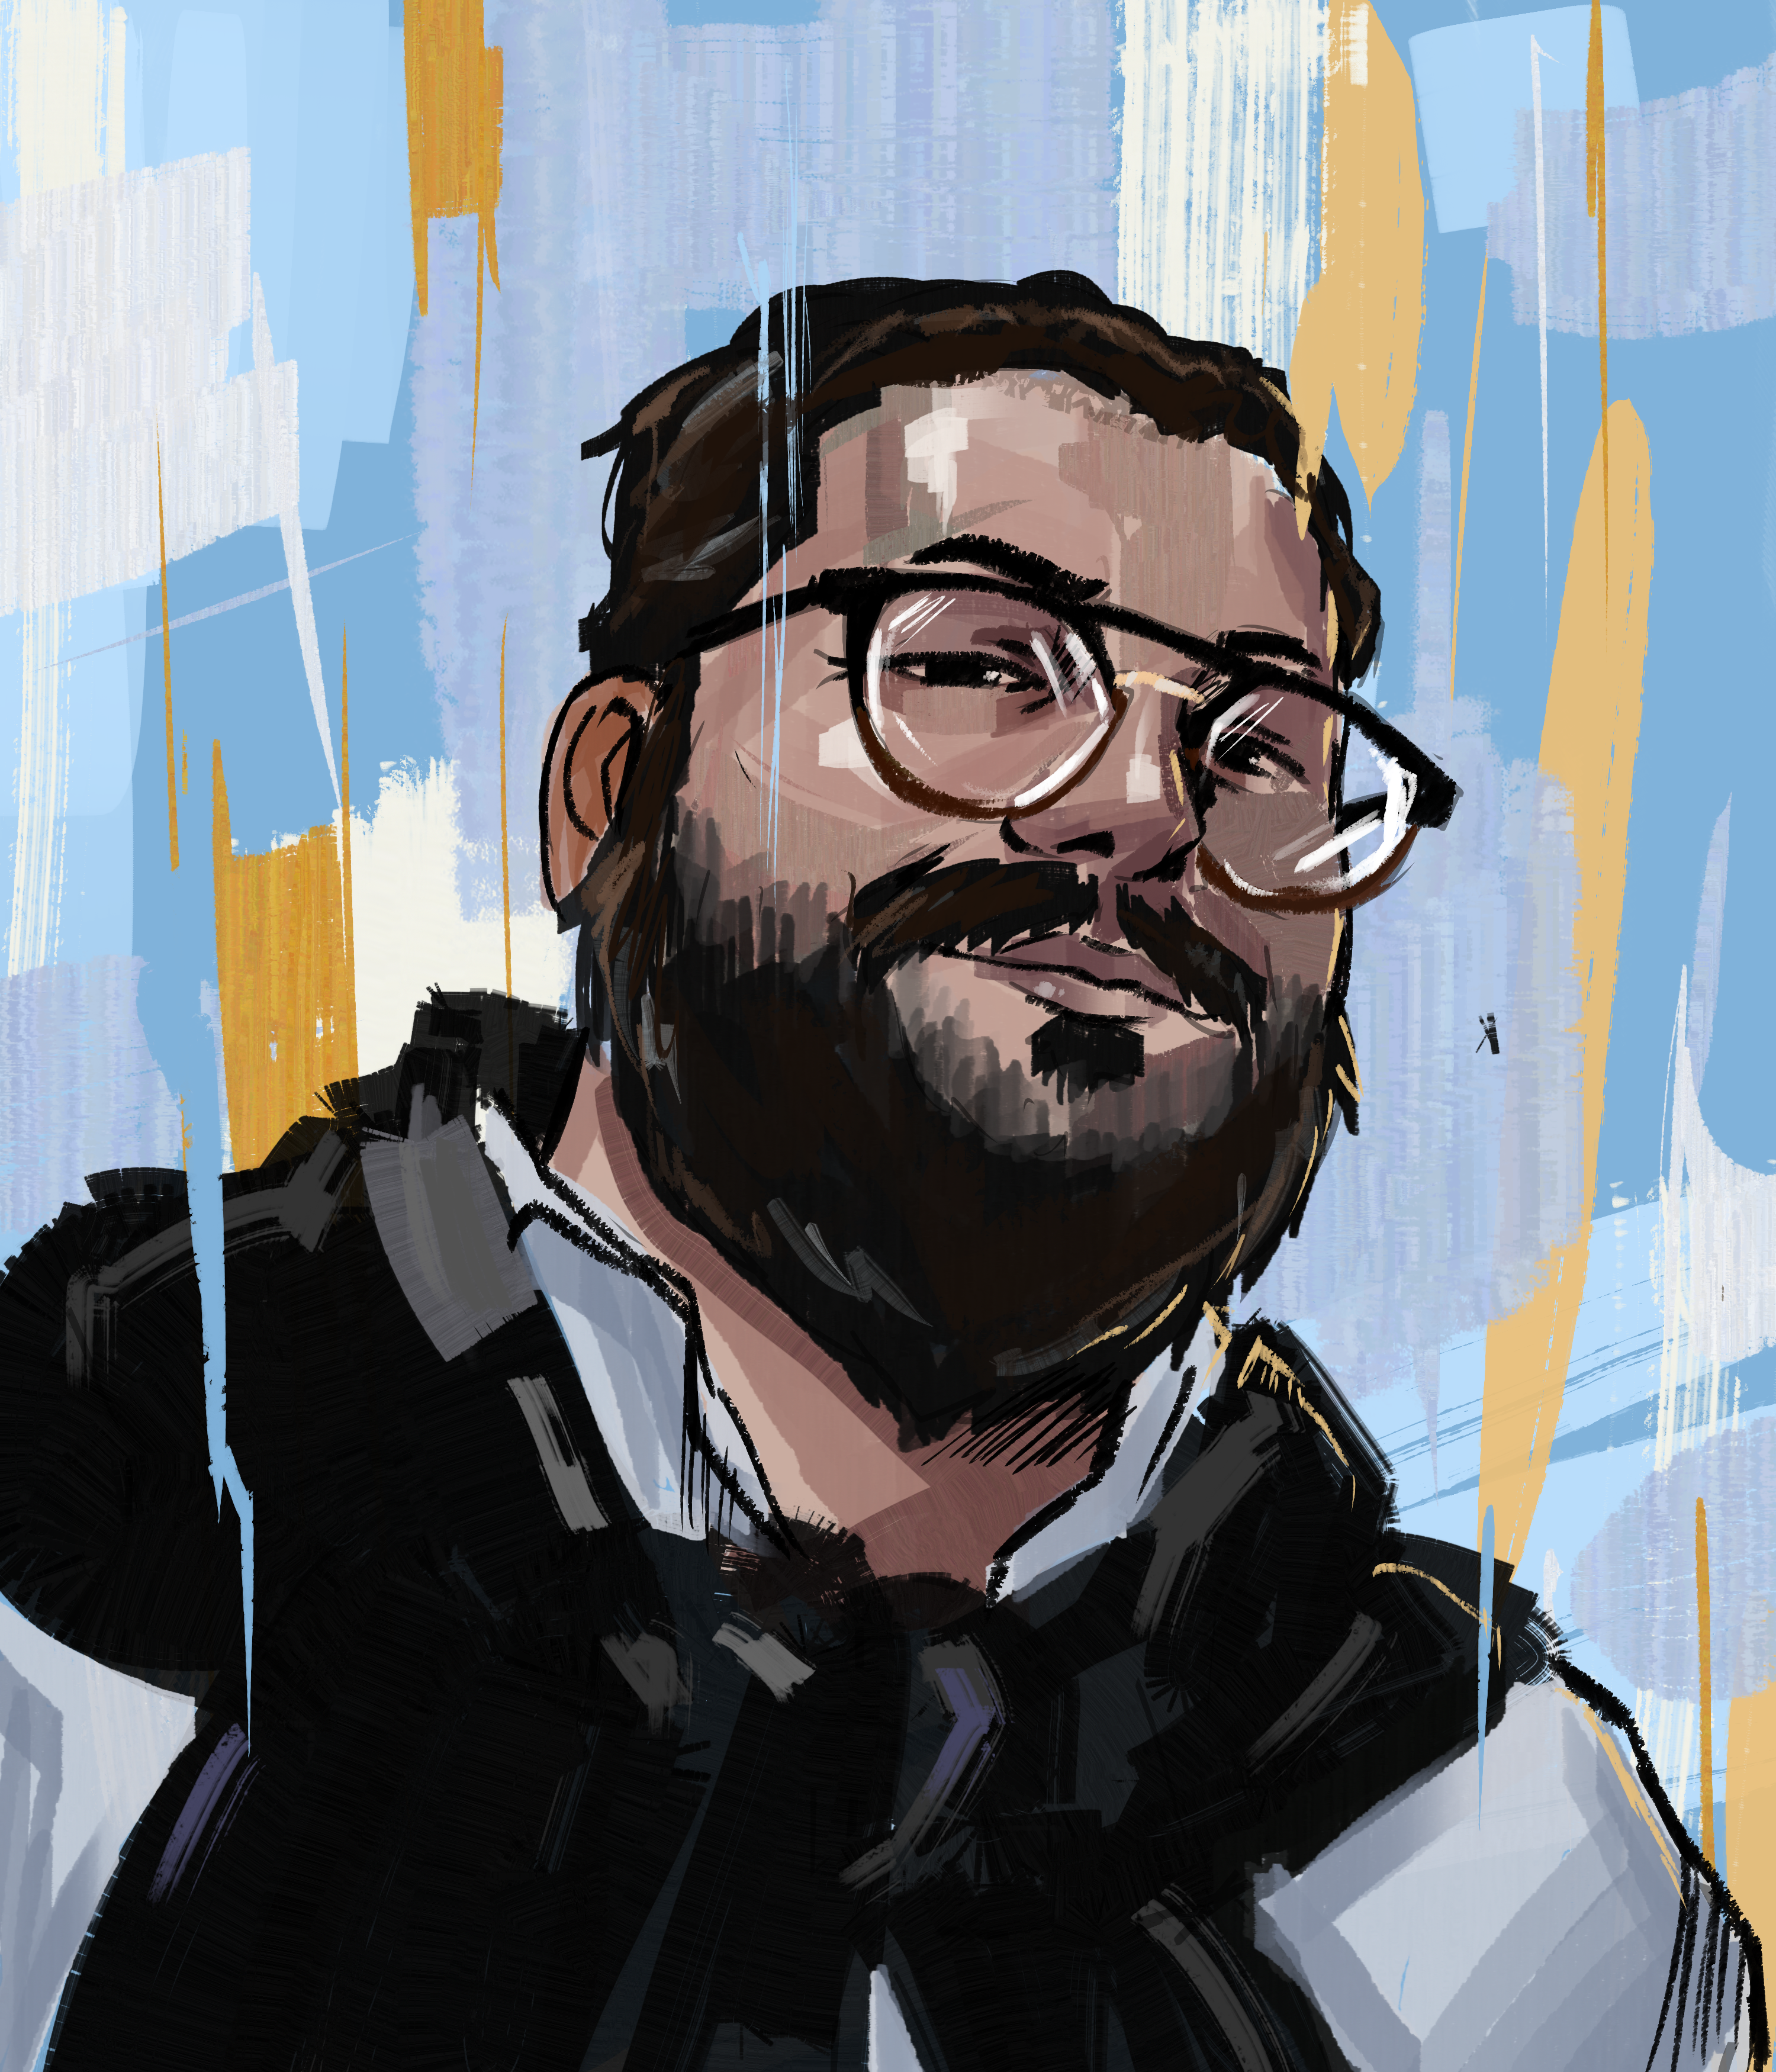
\includegraphics[scale=0.1]{max_3.png}}
\end{center}
\vfill


%%%%%%%%%%%
% CONTACT %
%%%%%%%%%%%
\clearpage
\section{Contact Information}
\begin{longtable}{p{4cm}p{11.5cm}}
   \textsc{Address}     & Carl von Ossietzky University of Oldenburg\\
                        & School of Humanities and Social Sciences\\
                        & Department of Philosophy\\
                        & Ammerländer Heerstraße 114\,--\,119\\
                        & 26129 Oldenburg\\
                        & Germany \\
                        & \\
   \textsc{Phone}       & +49 (0)441 798 2034\\
                        & \\
   \textsc{Email}      & \href{mailto:alexander.max.bauer@uol.de}{alexander.max.bauer@uol.de}\\
                        & \\
   \textsc{Website}     & \href{http://www.alexandermaxbauer.de/}{www.alexandermaxbauer.de}
\end{longtable}


%%%%%%%%%%%%%%%%%%%
% AREAS AND TOOLS %
%%%%%%%%%%%%%%%%%%%
\vspace{0.5cm}
\section{Areas and Tools}
\begin{longtable}{p{4cm}p{11.5cm}}
   \textsc{Areas of Specialisation}   & Experimental Philosophy, Need-Based Distributive Justice,\\
                                      & Causation\\
                                      & \\
   \textsc{Areas of Competence}       & Ludology, Distributive Justice, Philosophy of Science,\\
                                      & Metaphysics\\
                                      & \\
   \textsc{Areas of Interest}         & Digital Humanities, Metaphilosophy, Philosophy of Language\\
                                      & \\
   \textsc{Historical Focus}          & Aristotle, Friedrich Nietzsche\\
                                      & \\
   \textsc{Tools of Choice}           & \LaTeX, LimeSurvey, Stata, R, Python, Git
\end{longtable}


%%%%%%%%%%%%%%
% EMPLOYMENT %
%%%%%%%%%%%%%%
\clearpage
\section{Employment and Academic Path}
\begin{longtable}{p{2.5cm}p{11cm}}
\multirow{3}{2.5cm}{\footnotesize{09/2025\,--\,10/2025}} & Visiting Scholar\\
& \textsc{University of Zurich}\\
& \footnotesize{at the Department of Philosophy, working with Pascale Willemsen}\\
\\
\multirow{3}{2.5cm}{\footnotesize{06/2018\,--\,06/2022\\10/2022\,--\,04/2027}} & Research Associate\\
& \textsc{University of Oldenburg}\\
& \footnotesize{at the Department of Philosophy, working for Mark Siebel; 50 per cent from 06/2018 to 08/2019, 75 per cent from 09/2019 to 06/2021, 65 per cent from 07/2021 to 06/2022, and 50 per cent from 10/2022 to 04/2027; research in the project \enquote{Measures of Need-Based Justice, Expertise, and Coherence} of the research group \enquote{Need-Based Justice and Distribution Procedures} (FOR 2104) of the German Research Foundation (DFG) from 06/2018 to 06/2022}\\
\\
\multirow{3}{2.5cm}{\footnotesize{08/2017\,--\,12/2017}} & Research Associate\\
& \textsc{Helmut Schmidt University, University of the Federal Armed Forces}\\
& \footnotesize{at the Faculty of Economics and Social Sciences, working for Stefan Traub; 50 per cent; research in the project \enquote{Synergies of Behavioral Science and Game Analysis Research} as part of the program \enquote{Environmentally and Socially Compatible Transformation of the Energy System,} funded by the Federal Ministry of Education and Research (BMBF)}\\
\\
\multirow{3}{2.5cm}{\footnotesize{04/2017\,--\,03/2018\\10/2018\,--\,03/2020\\10/2022\,--\,03/2023\\10/2023\,--\,09/2024}} & Teaching Associate\\
& \textsc{University of Oldenburg}\\
& \footnotesize{at the Department of Philosophy; design and delivery of courses at bachelor's and master's level}\\
\\
\multirow{3}{2.5cm}{\footnotesize{02/2015\,--\,06/2018}} & Research Assistant\\
& \textsc{Karl-Jaspers-Gesellschaft e.\,V.}\\
& \footnotesize{working for Matthias Bormuth; from 04/2017 to 06/2018 on a self-employed basis; editing and lectoring of various book projects, finances and accounting, membership administration, as well as organisation and supervision of events}\\
\\
\multirow{3}{2.5cm}{\footnotesize{10/2013\,--\,06/2018}} & Research Assistant\\
& \textsc{University of Oldenburg}\\
& \footnotesize{at the Department of Philosophy, working for Mark Siebel, Martin Vialon, and Michael Städtler, as well as the Hannah-Arendt-Zentrum, working for Johann Kreuzer; conceptualisation and conduction of tutorial courses (theoretical and practical philosophy) and exercises (introduction to scientific work), organisation of a workshop and a symposium, and working in the project \enquote{Measures of Need-Based Justice, Expertise, and Coherence} of the research group \enquote{Need-Based Justice and Distribution Procedures} (FOR 2104) of the German Research Foundation (DFG)}\\
\\
\multirow{3}{2.5cm}{\footnotesize{04/2012\,--\,06/2013}} & Research Assistant\\
& \textsc{Institut für Ökonomische Bildung gGmbH}\\
& \footnotesize{working for Rudolf Schröder; maintaining contact with participants of empirical studies, processing of questionnaire data, preparation of statistical graphics, and support of a symposium}\\
\end{longtable}


%%%%%%%%%%%%%
% EDUCATION %
%%%%%%%%%%%%%
\clearpage
\section{Education}
\begin{longtable}{p{2.5cm}p{11cm}}
\multirow{3}{2.5cm}{\footnotesize{04/2017\,--\,02/2024}} & Doctor philosophiae (Philosophy)\\
& \textsc{University of Oldenburg}\\
& \footnotesize{passed with highest distinction (summa cum laude); cumulative thesis: \enquote{Empirische Studien zu Fragen der Bedarfsgerechtigkeit} (examiner: Mark Siebel, second examiner: Markus Tepe); date of the disputation: 14/02/2024 (further members of the commission: Dirk Büsch, Susanne Möbuß, and Mark Schweda)}\\
\\
\multirow{3}{2.5cm}{\footnotesize{04/2014\,--\,03/2017}} & Master of Arts (Philosophy)\\
& \textsc{University of Oldenburg}\\
& \footnotesize{passed with distinction (1,08); thesis: \enquote{Monotonie und Monotoniesensitivität als Desiderata für Maße der Bedarfsgerechtigkeit -- Zu zwei Aspekten der Grundlegung empirisch informierter Maße der Bedarfsgerechtigkeit zwischen normativer Theorie, formaler Modellierung und empirischer Sozialforschung} (examiner: Mark Siebel, second examiner: Arne Robert Weiss)}\\
\\
\multirow{3}{2.5cm}{\footnotesize{10/2010\,--\,03/2014}} & Bachelor of Arts (Politics and Economics, Philosophy)\\
& \textsc{University of Oldenburg}\\
& \footnotesize{passed with grade \enquote{very good} (1,47); thesis: \enquote{Friedrich Wilhelm Nietzsches Problematisierung von Sprache und Wahrheit in seiner Schrift \enquote{Ueber Wahrheit und Lüge im aussermoralischen Sinne}} (examiner: Johann Kreuzer, second examiner: Ingo Elbe)}\\
\\
\multirow{3}{2.5cm}{\footnotesize{08/2007\,--\,06/2010}} & Higher Education Entrance Qualification\\
& \textsc{Domgymnasium Verden}\\
& \footnotesize{passed with grade \enquote{good} (2,40); examination subjects with advanced requirement level: History, English, as well as Politics and Economics, examination subjects with basic requirement level: German and Physics}\\
\\
\multirow{3}{2.5cm}{\footnotesize{08/2004\,--\,06/2007}} & Extended Secondary School Qualification\\
& \textsc{Realschule Achim}\\
& \footnotesize{passed with grade \enquote{good} (2,30)}\\
\end{longtable}


%%%%%%%%%%%%%%%%
% PUBLICATIONS %
%%%%%%%%%%%%%%%%
\clearpage
\section{Publications}


%%%%%%%%%%%%%%%%%%
% IN PREPARATION %
%%%%%%%%%%%%%%%%%%
\subsection*{Manuscripts in Preparation or Under Review}
\begin{literature}
\lititem Henne, Paul; Pedryc, Wiktoria; Deichen, Benjamin; Bauer, Alexander Max; Sankner, Annika; Varghese, Saniya; Moonlight, Isaiah (under revision for \textit{New Ideas in Psychology}): \enquote{The Kraemer Effect Reconsidered.}

\lititem Schippers, Michael; Siebel, Mark; Kornmesser, Stephan; Bauer, Alexander Max (in preparation): \enquote{So Close and Yet So Far. Why Measures of Divergence and Similarity Make Bad Measures of Coherence.}

\lititem Bauer, Alexander Max; Kornmesser, Stephan; Alfano, Mark; Allard, Aurélien; Baumgartner, Lucien; Cova, Florian; Engelhardt, Paul; Fischer, Eugen; Meyer, Henrike; Reuter, Kevin; Sytsma, Justin; Thompson, Kyle; Wyszynski, Marc (in preparation): \textit{Experimentelle Philosophie. Eine Einführung in Methoden und Werkzeuge.} Berlin: J.\,B. Metzler.
\end{literature}


%%%%%%%%%%%%%%
% MONOGRAPHS %
%%%%%%%%%%%%%%
\subsection*{Monographs}
\begin{literature}
\lititem Bauer, Alexander Max (forthcoming): \textit{Empirical Studies on Questions of Need-Based Distributive Justice}. Paderborn: mentis.

\lititem Kornmesser, Stephan; Bauer, Alexander Max; Alfano, Mark; Allard, Aurélien; Baumgartner, Lucien; Cova, Florian; Engelhardt, Paul; Fischer, Eugen; Meyer, Henrike; Reuter, Kevin; Sytsma, Justin; Thompson, Kyle; Wyszynski, Marc (2024): \textit{Experimental Philosophy for Beginners. A Gentle Introduction to Methods and Tools}. Cham: Springer.

\lititem Bauer, Alexander Max (2024): \textit{Empirische Studien zu Fragen der Bedarfsgerechtigkeit}. Oldenburg: University of Oldenburg Press.
\end{literature}


%%%%%%%%%%%%%%%%%
% IN MONOGRAPHS %
%%%%%%%%%%%%%%%%%
\subsection*{Contributions to Monographs With Multiple Authors}
\begin{literature}
\lititem Bauer, Alexander Max; Kornmesser Stephan; Meyer, Henrike (2024): \enquote{Constative and Performative Utterances, $\chi^2$ Tests, and LimeSurvey.} In: Kornmesser, Stephan; Bauer, Alexander Max; Alfano, Mark; Allard, Aurélien; Baumgartner, Lucien; Cova, Florian; Engelhardt, Paul; Fischer, Eugen; Meyer, Henrike; Reuter, Kevin; Sytsma, Justin; Thompson, Kyle; Wyszynski, Marc: \textit{Experimental Philosophy for Beginners. A Gentle Introduction to Methods and Tools}. Cham: Springer.
\end{literature}


%%%%%%%%%%%%
% JOURNALS %
%%%%%%%%%%%%
\subsection*{Journals and Special Issues}
\begin{literature}
\lititem Bauer, Alexander Max; Ellmers, Sven; Nosthoff, Anna-Verena; Yildirim, Aylin (eds.) (in preparation): \textit{Oldenburger Philosophische Studien}.

\lititem Baratella, Nils; Bauer, Alexander Max; Grass, Helena Esther; Kornmesser, Stephan (eds.) (2022): \enquote{Verschwörungserzählungen.} Special issue of \textit{Zeitschrift für Praktische Philosophie} 9 (2).
\end{literature}


%%%%%%%%%%%%%%%
% IN JOURNALS %
%%%%%%%%%%%%%%%
\subsection*{Contributions to Journals}
\begin{literature}
\lititem Bauer, Alexander Max; Diederich, Adele; Traub, Stefan; Weiss, Arne Robert (2025): \enquote{Thinking About Need. A Vignette Experiment on Need-Based Distributive Justice.} \textit{The Journal of Economic Inequality}. (peer-reviewed)

\lititem Kornmesser, Stephan; Bauer, Alexander Max (2023): \enquote{Austin in the Lab. Empirically Reconsidering the Constative-Performative Distinction.} \textit{Topics in Linguistics} 24 (2), 1--14. (peer-reviewed)

\lititem Bauer, Alexander Max; Romann, Jan; Siebel, Mark; Traub, Stefan (2023): \enquote{Winter is Coming. How Laypeople Think About Different Kinds of Needs.} \textit{PLOS ONE} 18 (11), e0294572. (peer-reviewed)

\lititem Bauer, Alexander Max; Kornmesser, Stephan (2023): \enquote{Poisoned Babies, Shot Fathers, and Ruined Experiments. Experimental Evidence in Favor of the Compositionality Constraint of Actual Causation.} \textit{Philosophy of Science} 90 (3), 489--517. (peer-reviewed)

\lititem Wyszynski, Marc; Bauer, Alexander Max (2023): \enquote{Give What's Required and Take Only What You Need! The Effect of Framing on Rule-Breaking in Social Dilemmas.} \textit{Judgment and Decision Making} 18, e17. (peer-reviewed)

\lititem Bauer, Alexander Max; Meyer, Frauke; Romann, Jan; Siebel, Mark; Traub, Stefan (2022): \enquote{Need, Equity, and Accountability. Evidence on Third-Party Distribution Decisions from a Vignette Study.} \textit{Social Choice and Welfare} 59, 769--814. (peer-reviewed)

\lititem Bauer, Alexander Max; Romann, Jan (2022): \enquote{Answers at Gunpoint. On Livengood and Sytsma's Revolver Case.} \textit{Philosophy of Science} 89 (1), 180--192. (peer-reviewed)

\lititem Bauer, Alexander Max (2022): \enquote{Sated but Thirsty. A Prolegomenon to Multidimensional Measures of Need-Based Justice.} \textit{Axiomathes} 32, 529--538. (peer-reviewed)

\lititem Bauer, Alexander Max (2021): \enquote{Christian Neuhäuser. Wie reich darf man sein? Über Gier, Neid und Gerechtigkeit.} \textit{Zeitschrift für philosophische Forschung} 75 (1), 160--164.

\lititem Bauer, Alexander Max (2019): \enquote{Christian Neuhäuser. Reichtum als moralisches Problem.} \textit{Zeitschrift für Ethik und Moralphilosophie} 2 (2), 381--385.

\lititem Bauer, Alexander Max (2017): \enquote{Axiomatic Foundations for Metrics of Distributive Justice Shown by the Example of Needs-Based Justice.} \textit{\enquote{forsch!} -- Studentisches Online-Journal der Universität Oldenburg} 3 (1), 43--60. (peer-reviewed)

\lititem Bauer, Alexander Max (2017): \enquote{Axiomatische Überlegungen zu Grundlagen für Maße der Verteilungsgerechtigkeit am Beispiel von Bedarfsgerechtigkeit.} \textit{\enquote{forsch!} -- Studentisches Online-Journal der Universität Oldenburg} 3 (1), 23--42. (peer-reviewed)

\lititem Bauer, Alexander Max; Meyerhuber, Malte Ingo (2016): \enquote{Über die Frage, ob wir uns dazu entscheiden können, etwas zu glauben. Wider eines idealisierten Verständnisses des doxastischen Voluntarismus.} \textit{\enquote{forsch!} -- Studentisches Online-Journal der Universität Oldenburg} 2 (2), 10--21. (peer-reviewed)
\end{literature}


%%%%%%%%%%%%%%%%%%
% EDITED VOLUMES %
%%%%%%%%%%%%%%%%%%
\subsection*{Edited Volumes}
\begin{literature}
\lititem Bauer, Alexander Max; Grass, Helena Esther (eds.) (2024): \textit{Oldenburger Jahrbuch für Philosophie 2021/2022}. Oldenburg: University of Oldenburg Press.

\lititem Bauer, Alexander Max; Damschen, Gregor; Siebel, Mark (eds.) (2023): \textit{Paradoxien. Grenzdenken und Denkgrenzen von A(llwissen) bis Z(eit)}. Paderborn: mentis.

\lititem Bauer, Alexander Max; Kornmesser, Stephan (eds.) (2023): \textit{The Compact Compendium of Experimental Philosophy}. Berlin and Boston: Walter de Gruyter.

\lititem Bauer, Alexander Max; Baratella, Nils (eds.) (2021): \textit{Oldenburger Jahrbuch für Philosophie 2019/2020}. Oldenburg: BIS-Verlag.

\lititem Bauer, Alexander Max; Meyerhuber, Malte Ingo (eds.) (2020): \textit{Empirical Research and Normative Theory. Transdisciplinary Perspectives on Two Methodical Traditions Between Separation and Interdependence}. Berlin and Boston: Walter de Gruyter. (paperback edition 2021)

\lititem Bauer, Alexander Max; Meyerhuber, Malte Ingo (eds.) (2019): \textit{Philosophie zwischen Sein und Sollen. Normative Theorie und empirische Forschung im Spannungsfeld}. Berlin and Boston: Walter de Gruyter. (paperback edition 2021)

\lititem Bauer, Alexander Max; Baratella, Nils (eds.) (2019): \textit{Oldenburger Jahrbuch für Philosophie 2017/2018}. Oldenburg: BIS-Verlag.
\end{literature}


%%%%%%%%%%%%%%%%%%%%%
% IN EDITED VOLUMES %
%%%%%%%%%%%%%%%%%%%%%
\subsection*{Contributions to Edited Volumes}
\begin{literature}
\lititem Bauer, Alexander Max; Romann, Jan (2024): \enquote{Equal Deeds, Different Needs. Need, Accountability, and Resource Availability in Third-Party Distribution Decisions.} In: Knobe, Joshua; Nichols, Shaun (eds.): \textit{Oxford Studies in Experimental Philosophy}. Vol. 5. Oxford: Oxford University Press. 7--31. (peer-reviewed)

\lititem Bauer, Alexander Max; Siebel, Mark (2024): \enquote{Measuring Need-Based Justice. Empirically and Formally.} In: Kittel, Bernhard; Traub, Stefan (eds.): \textit{Priority of Needs? An Informed Theory of Need-Based Justice}. Cham: Springer. 61--94.

\lititem Bauer, Alexander Max (2021): \enquote{Babylonische Befindlichkeiten. Hans-Helmuth Bruns' \enquote{Babel in Deutschland}.} In: Bauer, Alexander Max; Baratella, Nils (eds.): \textit{Oldenburger Jahrbuch für Philosophie 2019/2020}. Oldenburg: BIS-Verlag. 283--290.

\lititem Bauer, Alexander Max; Meyerhuber, Malte Ingo (2020): \enquote{Two Worlds on the Brink of Colliding. On the Relationship Between Empirical Research and Normative Theory.} In: id. (eds.): \textit{Empirical Research and Normative Theory. Transdisciplinary Perspectives on Two Methodical Traditions Between Separation and Interdependence}. Berlin and Boston: Walter de Gruyter. 11--33.

\lititem Bauer, Alexander Max (2019): \enquote{Zur Grundlegung empirisch informierter Maße der Bedarfsgerechtigkeit. Zwei Desiderata zwischen normativer Theorie, formaler Modellierung und empirischer Sozialforschung.} In: Bauer, Alexander Max; Meyerhuber, Malte Ingo (eds.): \textit{Philosophie zwischen Sein und Sollen. Normative Theorie und empirische Forschung im Spannungsfeld}. Berlin and Boston: Walter de Gruyter. 179--220.

\lititem Bauer, Alexander Max; Meyerhuber, Malte Ingo (2019): \enquote{Zwei Welten am Rande der Kollision. Zum Verhältnis von empirischer Forschung und normativer Theorie, insbesondere vor dem Hintergrund der Ethik.} In: id. (eds.): \textit{Philosophie zwischen Sein und Sollen. Normative Theorie und empirische Forschung im Spannungsfeld}. Berlin and Boston: Walter de Gruyter. 13--37.

\lititem Bauer, Alexander Max (2019): \enquote{\enquote{Wahrheit ist, was uns verbindet.} Den Absolventinnen und Absolventen der Fakultät IV zum Geleit.} In: Bauer, Alexander Max; Baratella, Nils (eds.): \textit{Oldenburger Jahrbuch für Philosophie 2017/2018}. Oldenburg: BIS-Verlag. 353--357.

\lititem Bauer, Alexander Max (2019): \enquote{Gerechtigkeit und Bedürfnis. Perspektiven auf den Begriff des \enquote{Bedürfnisses} vor dem Hintergrund der Bedarfsgerechtigkeit.} In: Bauer, Alexander Max; Baratella, Nils (eds.): \textit{Oldenburger Jahrbuch für Philosophie 2017/2018}. Oldenburg: BIS-Verlag. 285--327.
\end{literature}


%%%%%%%%%%%%
% PREFACES %
%%%%%%%%%%%%
\subsection*{Prefaces, Introductions, and Epilogues}
\begin{literature}
\lititem Kornmesser, Stephan; Bauer, Alexander Max; Alfano, Mark; Allard, Aurélien; Baumgartner, Lucien; Cova, Florian; Engelhardt, Paul; Fischer, Eugen; Meyer, Henrike; Reuter, Kevin; Sytsma, Justin; Thompson, Kyle; Wyszynski, Marc (2024): \enquote{Introduction. Setting Out For New Shores.} In: id. (eds.): \textit{Experimental Philosophy for Beginners. A Gentle Introduction to Methods and Tools}. Cham: Springer. 1--18.

\lititem Grass, Helena Esther; Bauer, Alexander Max (2024): \enquote{Vorwort.} In: Bauer, Alexander Max; Grass, Helena Esther (eds.): \textit{Oldenburger Jahrbuch für Philosophie 2021/2022}. Oldenburg: University of Oldenburg Press. 7--10.

\lititem Bauer, Alexander Max; Damschen, Gregor; Siebel, Mark (2023): \enquote{Vorwort.} In: id. (eds.): \textit{Paradoxien. Grenzdenken und Denkgrenzen von A(llwissen) bis Z(eit)}. Paderborn: mentis. VII--XIII.

\lititem Kornmesser, Stephan; Bauer, Alexander Max (2023): \enquote{Introduction.} In: Bauer, Alexander Max; Kornmesser, Stephan (eds.): \textit{The Compact Compendium of Experimental Philosophy}. Berlin and Boston: Walter de Gruyter. 1--5.

\lititem Baratella, Nils; Bauer, Alexander Max; Grass, Helena Esther; Kornmesser, Stephan (2022): \enquote{Einleitung. Verschwörungserzählungen.} \textit{Zeitschrift für Praktische Philosophie} 9 (2), 105--112.

\lititem Bauer, Alexander Max; Baratella, Nils (2021): \enquote{Vorwort.} In: id. (eds.): \textit{Oldenburger Jahrbuch für Philosophie 2019/2020}. Oldenburg: BIS-Verlag. 5.

\lititem Bauer, Alexander Max; Meyerhuber, Malte Ingo (2020): \enquote{Epilogue. On Doxa and Aletheia.} In: id. (eds.): \textit{Empirical Research and Normative Theory. Transdisciplinary Perspectives on Two Methodical Traditions Between Separation and Interdependence}. Berlin and Boston: Walter de Gruyter. 337--342.

\lititem Bauer, Alexander Max; Meyerhuber, Malte Ingo (2020): \enquote{Introduction.} In: id. (eds.): \textit{Empirical Research and Normative Theory. Transdisciplinary Perspectives on Two Methodical Traditions Between Separation and Interdependence}. Berlin and Boston: Walter de Gruyter. 1--10.

\lititem Bauer, Alexander Max; Meyerhuber, Malte Ingo (2020): \enquote{Preface.} In: id. (eds.): \textit{Empirical Research and Normative Theory. Transdisciplinary Perspectives on Two Methodical Traditions Between Separation and Interdependence}. Berlin and Boston: Walter de Gruyter. VII--VIII.

\lititem Bauer, Alexander Max; Meyerhuber, Malte Ingo (2019): \enquote{Epilog. Zwischen doxa und aletheia.} In: id. (eds.): \textit{Philosophie zwischen Sein und Sollen. Normative Theorie und empirische Forschung im Spannungsfeld}. Berlin und Boston: Walter de Gruyter. 221--225.

\lititem Bauer, Alexander Max; Meyerhuber, Malte Ingo (2019): \enquote{Einleitung.} In: id. (eds.): \textit{Philosophie zwischen Sein und Sollen. Normative Theorie und empirische Forschung im Spannungsfeld}. Berlin and Boston: Walter de Gruyter. 1--11.

\lititem Bauer, Alexander Max; Meyerhuber, Malte Ingo (2019): \enquote{Vorwort.} In: id. (eds.): \textit{Philosophie zwischen Sein und Sollen. Normative Theorie und empirische Forschung im Spannungsfeld}. Berlin and Boston: Walter de Gruyter. XI--XII.

\lititem Bauer, Alexander Max; Baratella, Nils (2019): \enquote{Vorwort.} In: id. (eds.): \textit{Oldenburger Jahrbuch für Philosophie 2017/2018}. Oldenburg: BIS-Verlag. 5.
\end{literature}


%%%%%%%%%%%%%%%%%%
% WORKING PAPERS %
%%%%%%%%%%%%%%%%%%
\subsection*{Working Papers}
\begin{literature}
\lititem Henne, Paul; Pedryc, Wiktoria; Deichen, Benjamin; Bauer, Alexander Max; Sankner, Annika; Varghese, Saniya; Moonlight, Isaiah (2025): \enquote{The Kraemer Effect Reconsidered.} \textit{OSF Preprints}.

\lititem Bauer, Alexander Max; Diederich, Adele; Traub, Stefan; Weiss, Arne Robert (2023): \enquote{Thinking About Need. A Vignette Experiment on Need-Based Distributive Justice.} \textit{SSRN Working Paper} 4503209.

\lititem Bauer, Alexander Max; Romann, Jan; Siebel, Mark; Traub, Stefan (2023): \enquote{Winter is Coming. How Laypeople Think About Different Kinds of Needs.} \textit{SSRN Working Paper} 4383555.

\lititem Wyszynski, Marc; Bauer, Alexander Max (2022): \enquote{Give What You Can, Take What You Need. The Effect of Framing on Rule-Breaking Behavior in Social Dilemmas.} \textit{FOR 2104 Working Paper} 2022--01.

\lititem Bauer, Alexander Max; Meyer, Frauke; Romann, Jan; Siebel, Mark; Traub, Stefan (2020): \enquote{Need, Equity, and Accountability. Evidence on Third-Party Distributive Decisions from an Online Experiment.} \textit{FOR 2104 Working Paper} 2020--01.

\lititem Bauer, Alexander Max (2018): \enquote{Sated but Thirsty. Towards a Multidimensional Measure of Need-Based Justice.} \textit{FOR 2104 Working Paper} 2018--03.

\lititem Bauer, Alexander Max (2018): \enquote{Monotonie und Monotoniesensitivität als Desiderata für Maße der Bedarfsgerechtigkeit. Zu zwei Aspekten der Grundlegung empirisch informierter Maße der Bedarfsgerechtigkeit zwischen normativer Theorie, formaler Modellierung und empirischer Sozialforschung.} \textit{FOR 2104 Working Paper} 2018--01.

\lititem Weiss, Arne Robert; Bauer, Alexander Max; Traub, Stefan (2017): \enquote{Needs as Reference Points. When Marginal Gains to the Poor do not Matter.} \textit{FOR 2104 Working Paper} 2017--13.

\lititem Traub, Stefan; Bauer, Alexander Max; Siebel, Mark; Springhorn, Nils; Weiss, Arne Robert (2017): \enquote{On the Measurement of Need-Based Justice.} \textit{FOR 2104 Working Paper} 2017--12.
\end{literature}


%%%%%%%%%%%%%%%%
% TRANSLATIONS %
%%%%%%%%%%%%%%%%
\subsection*{Translations}
\begin{literature}
\lititem Priest, Graham (2023): \enquote{Paradoxie und Parakonsistenz.} Transl. by Bauer, Alexander Max; Damschen, Gregor; Siebel, Mark. In: id. (eds.): \textit{Paradoxien. Grenzdenken und Denkgrenzen von A(llwissen) bis Z(eit)}. Paderborn: mentis. 225--248.
\end{literature}


%%%%%%%%%%%%%%%%
% DISSERTATION %
%%%%%%%%%%%%%%%%
\subsection*{Dissertation}
\begin{literature}
\lititem Bauer, Alexander Max (2024): \textit{Empirische Studien zu Fragen der Bedarfsgerechtigkeit.} Dissertation. University of Oldenburg.
\end{literature}


%%%%%%%%%%%%%%%%%
% PRESENTATIONS %
%%%%%%%%%%%%%%%%%
\clearpage
\section{Presentations}


%%%%%%%%%%%
% INVITED %
%%%%%%%%%%%
\subsection*{Invited}
\begin{longtable}{p{2.5cm}p{11cm}}
\multirow{2}{2.5cm}{\footnotesize{20/07/2024}} & Poisoned Babies, Shot Fathers, and Ruined Experiments -- Experimental Evidence in Favor of the Compositionality Constraint of Actual Causation\\
& \footnotesize{presentation at the 2nd meeting of the Society for Philosophy of Causation; University of Göttingen; invited by Tom Wysocki}\\
\\
\multirow{2}{2.5cm}{\footnotesize{08/12/2017}} & Mind the Gap -- Zur Vermittlung von normativer Theorie und empirischer Forschung\\
& \footnotesize{presentation at the lecture series \enquote{Junge Philosophie}; Karl-Jaspers-Gesellschaft in Oldenburg; jointly with Malte Ingo Meyerhuber; invited by Ansgar Baumgart, Malte Maria Unverzagt, and Philip Penew}\\
\\
\multirow{2}{2.5cm}{\footnotesize{22/11/2016}} & Grundlagen für Maße der Bedarfsgerechtigkeit -- Axiomatische Überlegungen und empirische Untersuchungen\\
& \footnotesize{presentation at the Department of Philosophy's colloquium; University of Oldenburg; jointly with Arne Robert Weiss; invited by Nils Baratella}\\
\end{longtable}


%%%%%%%%%%%%
% REVIEWED %
%%%%%%%%%%%%
\subsection*{Reviewed}
\begin{longtable}{p{2.5cm}p{11cm}}
\multirow{2}{2.5cm}{\footnotesize{12/07/2025}} & Empirical Studies on Questions of Need-Based Distributive Justice\\
& \footnotesize{presentation at the 5th European Experimental Philosophy Conference; University of East Anglia}\\
\\
\multirow{2}{2.5cm}{\footnotesize{20/06/2025}} & The Kraemer Effect Reconsidered\\
& \footnotesize{poster presentation at the 51st Annual Meeting of the Society for Philosophy \& Psychology; Cornell University; jointly with Paul Henne, Wiktoria Pedryc, Benjamin Deichen, Annika Sankner, Saniya Varghese, and Isaiah Moonlight}\\
\\
\multirow{2}{2.5cm}{\footnotesize{16/09/2023}} & Poisoned Babies, Shot Fathers, and Ruined Experiments -- Experimental Evidence in Favor of the Compositionality Constraint of Actual Causation\\
& \footnotesize{presentation at the 3rd European Experimental Philosophy Conference; University of Zurich; attended online due to funding problems}\\
\\
\multirow{2}{2.5cm}{\footnotesize{07/09/2021}} & Need and Responsibility -- Experimental Philosophy Investigating Questions of Distributive Justice\\
& \footnotesize{presentation at the 25th Congress of the German Society for Philosophy (DGPhil); Friedrich-Alexander University Erlangen-Nürnberg; held online due to pandemic}\\
\\
\multirow{2}{2.5cm}{\footnotesize{23/08/2021}} & Give What You Can, Take What You Need -- The Effect of Framing on Fraudulent Behavior in Social Dilemmas\\
& \footnotesize{poster presentation at the Subjective Probability, Utility, and Decision Making Conference; University of Warwick; jointly with Marc Wyszynski; held online due to pandemic}\\
\\
\multirow{2}{2.5cm}{\footnotesize{07/2021}} & Need and Responsibility -- Experimental Philosophy on Questions of Distributive Justice\\
& \footnotesize{presentation accepted for the 18th Biennial Conference of the International Society for Justice Research; Católica Lisbon School of Business \& Economics; not attended due to unforeseen circumstances}\\
\\
\multirow{2}{2.5cm}{\footnotesize{18/06/2021}} & Austin in the Lab -- Experimental Evidence in Favor of the Constative-Performative Distinction\\
& \footnotesize{poster presentation and blitz talk at the 1st European Experimental Philosophy Conference; Charles University in Prague; jointly with Stephan Kornmesser; held online due to pandemic}\\
\\
\multirow{2}{2.5cm}{\footnotesize{10/2020}} & Valides Werkzeug oder bloßes Rechenspiel? Zur moralischen Aussagekraft von Gedankenexperimenten\\
& \footnotesize{presentation accepted for the 8th Conference for Practical Philosophy; University of Salzburg; jointly with Malte Ingo Meyerhuber und Jan Romann; cancelled due to pandemic}\\
\\
\multirow{2}{2.5cm}{\footnotesize{24/07/2020}} & Need and Responsibility\\
& \footnotesize{presentation at the annual conference of the Society for the Advancement of Behavioral Economics; National Research University, Higher School of Economics, Moscow; held online due to pandemic}\\
\\
\multirow{2}{2.5cm}{\footnotesize{21/06/2020}} & Need and Responsibility -- Experimental Philosophy on Questions of Distributive Justice\\
& \footnotesize{presentation at the 1st European Experimental Philosophy Conference; Charles University in Prague; held online due to pandemic}\\
\\
\multirow{2}{2.5cm}{\footnotesize{05/2020}} & Need and Responsibility -- Experimental Philosophy on Questions of Distributive Justice\\
& \footnotesize{presentation accepted for the 20th International Conference on Moral and Political Philosophy; Universitat de les Illes Balears; cancelled due to pandemic}\\
\\
\multirow{2}{2.5cm}{\footnotesize{16/06/2019}} & Modern Day Ethics Between Empirical Research and Normative Theory\\
& \footnotesize{presentation at the Swedish Congress of Philosophy (Filosofidagarna); Umeå Universitet}\\
\\
\multirow{2}{2.5cm}{\footnotesize{05/04/2019}} & Experiments on Needs-Based Justice -- When Marginal Gains to the Poor do not Matter\\
& \footnotesize{presentation at the 12th Annual University at Albany Philosophical Association Graduate Conference \enquote{Rage Against the Armchair}; University at Albany, The State University of New York; commented by Sydney Faught}\\
\\
\multirow{2}{2.5cm}{\footnotesize{08/12/2018}} & Empirisch informierte Indizes der Bedarfsgerechtigkeit -- Zu dem Versuch, Bedarfsgerechtigkeit zwischen normativer Theorie, mathematischer Formalisierung und empirischer Sozialforschung zu operationalisieren\\
& \footnotesize{presentation at the 10th Doctoral Student's Symposium of the Austrian Philosophical Society (ÖGP); University of Klagenfurt}\\
\\
\multirow{2}{2.5cm}{\footnotesize{05/05/2018}} & Positive Psychologie zwischen empirischer Forschung und normativer Theorie\\
& \footnotesize{presentation at the 3rd Conference of the German Society for Positive Psychological Research (DGPPF); Ruhr University Bochum; jointly with Malte Ingo Meyerhuber}\\
\\
\multirow{2}{2.5cm}{\footnotesize{08/06/2016}} & Empirisch informierte Maße der Bedarfsgerechtigkeit -- Zwischen normativer Theorie, mathematischer Formalisierung und empirischer Sozialforschung\\
& \footnotesize{presentation at the congress of undergraduate research \enquote{forschen@studium}; University of Oldenburg}\\
\end{longtable}


%%%%%%%%%%
% OTHERS %
%%%%%%%%%%
\clearpage % tmp %
\subsection*{Others}
\begin{longtable}{p{2.5cm}p{11cm}}
\multirow{2}{2.5cm}{\footnotesize{03/06/2025}} & Distributive Justice and Reference Points\\
& \footnotesize{presentation at the lab meeting of the Experimental Philosophy Group; University of Zurich; attended online}\\
\\
\multirow{2}{2.5cm}{\footnotesize{14/02/2024}} & Empirische Studien zu Fragen der Bedarfsgerechtigkeit\\
& \footnotesize{doctoral dissertation defence; University of Oldenburg}\\
\\
\multirow{2}{2.5cm}{\footnotesize{22/05/2022}} & Measuring Need-Based Distributive Justice Normatively and Empirically\\
& \footnotesize{poster presentation at the Symposium on Need-Based Justice of the research group \enquote{Need-Based Justice and Distribution Procedures} (FOR 2104) of the German Research Foundation (DFG); University of Hamburg; jointly with Mark Siebel}\\
\\
\multirow{2}{2.5cm}{\footnotesize{14/02/2020}} & Types of Need\\
& \footnotesize{presentation at the workshop of the academic assistants of the research group \enquote{Need-Based Justice and Distribution Procedures} (FOR 2104) of the German Research Foundation (DFG); Jacobs University Bremen}\\
\\
\multirow{2}{2.5cm}{\footnotesize{12/02/2020}} & Need and Responsibility\\
& \footnotesize{presentation at the meeting of the research group \enquote{Need-Based Justice and Distribution Procedures} (FOR 2104) of the German Research Foundation (DFG); Jacobs University Bremen}\\
\\
\multirow{2}{2.5cm}{\footnotesize{22/11/2018}} & What Makes a Theory of Justice \enquote{Empirically Informed}? On the Possibilities and Impossibilities of Integrating Empirical Research Into Normative Theory\\
& \footnotesize{presentation at the workshop of the academic assistants of the research group \enquote{Need-Based Justice and Distribution Procedures} (FOR 2104) of the German Research Foundation (DFG); University of Bremen}\\
\\
\multirow{2}{2.5cm}{\footnotesize{16/02/2018}} & \enquote{Wahrheit ist, was uns verbindet}\\
& \footnotesize{address at the graduation ceremony of the School of Humanities and Social Sciences; University of Oldenburg}\\
\\
\multirow{2}{2.5cm}{\footnotesize{14/12/2017}} & Comparative and Non-Comparative Justice -- An Experimental Investigation in the Domain of Needs-Based Justice\\
& \footnotesize{presentation at the workshop of the academic assistants of the research group \enquote{Need-Based Justice and Distribution Procedures} (FOR 2104) of the German Research Foundation (DFG); University of Oldenburg; jointly with Nils Springhorn}\\
\\
\multirow{2}{2.5cm}{\footnotesize{14/12/2017}} & Empirische interkulturelle Forschung zur Evaluation von Bedarfsgerechtigkeit vor dem Hintergrund von sozialisationsbedingten Verzerrungen\\
& \footnotesize{presentation at the workshop of the academic assistants of the research group \enquote{Need-Based Justice and Distribution Procedures} (FOR 2104) of the German Research Foundation (DFG); University of Oldenburg}\\
\\
\multirow{2}{2.5cm}{\footnotesize{28/10/2017}} & Empirische Forschung und normative Theorie -- Eine Problembestimmung\\
& \footnotesize{presentation at the summer school \enquote{Empirical Research and Normative Theory} at the \enquote{Oldenburg School for the Social Sciences and the Humanities 2017} of the Graduate School for the Social Sciences and the Humanities (3GO); University of Oldenburg; jointly with Malte Ingo Meyerhuber}\\
\\
\\ % tmp %
\\ % tmp %
\multirow{2}{2.5cm}{\footnotesize{12/02/2016}} & Entwicklung eines empirisch gestützen Maßes der Bedarfsgerechtigkeit -- Ein axiomatischer Ansatz\\
& \footnotesize{presentation at the meeting of the research group \enquote{Need-Based Justice and Distribution Procedures} (FOR 2104) of the German Research Foundation (DFG); Hanse-Wissenschaftskolleg, Institute for Advanced Study (HWK) in Delmenhorst; jointly with Mark Siebel}\\
\\
\multirow{2}{2.5cm}{\footnotesize{07/07/2015}} & Mögliche Maße der Bedarfsgerechtigkeit -- Überlegungen zu Vektoren und Logarithmen\\
& \footnotesize{presentation at Mark Siebel's graduation colloquium; University of Oldenburg}\\
\end{longtable}


%%%%%%%%%%
% EVENTS %
%%%%%%%%%%
\clearpage
\section{Events}
\begin{longtable}{p{2.5cm}p{11cm}}
\multirow{3}{2.5cm}{\footnotesize{Summer 2022\\Winter 2022/2023\\Summer 2023\\Winter 2023/2024\\Summer 2024\\Winter 2024/2025}} & Philosophisches Kolloquium\\
& \footnotesize{the Department of Philosophy's colloquium; University of Oldenburg; organised jointly with Helena Esther Grass (summer 2022), Gesa Wellmann (summer 2023 -- winter 2024/2025), Tilo Wesche (summer 2022 -- winter 2024/2025), Malte Maria Unverzagt (winter 2024/2025), and Matthias Bormuth (winter 2024/2025)}\\
& \footnotesize{featuring contributions by Monika Albrecht, Niklas Angebauer, Dagmar Borchers, Alexandra Colligs, Gregor Damschen, Karin de Boer, Mitchell Dean, Kristina Engelhard, Bärbel Frischmann, Michael Hampe, Hilkje Hänel, Georg Hartmann, Timo Heisenberg, Lisa Herzog, Maximilian Kiener, Dagmar Kiesel, Kristina Lepold, Thomas Meyer, Elif Özmen, Ludger Schwarte, Sebastian Spanknebel, Titus Stahl, Malte Maria Unverzagt, Barbara Vetter, Ulrich von Bülow, Eva Weiler, Gesa Wellmann, and Tilo Wesche}\\
\\
\multirow{3}{2.5cm}{\footnotesize{Summer 2021}} & Nur Fußnoten zu Platon?\\
& \footnotesize{lecture series; University of Oldenburg; organised jointly with Gregor Damschen, Stephan Kornmesser, and Mark Siebel}\\
& \footnotesize{featuring contributions by Rafael Ferber, Jörg Hardy, Christoph Helmig, Joachim Horvath, Mark Textor, and Emanuel Viebahn}\\
\\
\multirow{3}{2.5cm}{\footnotesize{Winter 2019/2020}} & Paradoxien\\
& \footnotesize{lecture series; University of Oldenburg; organised jointly with Gregor Damschen and Mark Siebel}\\
& \footnotesize{featuring contributions by Inga Bones, Elke Brendel, Gregor Damschen, Guido Kreis, Paul Näger, Mark Siebel, Norman Sieroka, and Stefan Uppenkamp}\\
\\
\multirow{3}{2.5cm}{\footnotesize{13\,--\,15/12/2017}} & Workshop der Wissenschaftlichen Mitarbeiter\\
& \footnotesize{workshop of the academic assistants of the research group \enquote{Need-Based Justice and Distribution Procedures} (FOR 2104) of the German Research Foundation (DFG); Karl-Jaspers-Haus in Oldenburg; organised jointly with Maximilian Lutz, Fabian Paetzel, Nils Springhorn, and Arne Robert Weiss}\\
& \footnotesize{featuring contributions by Meike Benker, Marina Chugunova, Andrew Lawrence Fassett, Jan Philipp Krügel, Sabine Neuhofer, Manuel Schwaninger, Marc Wyszynski, and Patricia Zauchner, as well as a method workshop by Michael Jankowski}\\
\\
\multirow{3}{2.5cm}{\footnotesize{28\,--\,29/09/2017}} & Empirical Research and Normative Theory\\
& \footnotesize{international summer school at the \enquote{Oldenburg School for the Social Sciences and the Humanities 2017} of the Graduate School for the Social Sciences and the Humanities (3GO); University of Oldenburg; organised jointly with Malte Ingo Meyerhuber and Rea Kodalle}\\
& \footnotesize{featuring contributions by Max Agostini, Martijn Boot, Maarten Derksen, Niklas Dworazik, Carlos de Matos Fernandes, Andrea Klonschinski, Jannis Kreienkamp, Marvin Kunz, Bert Musschenga, Elsa Romfeld, Hanno Sauer, Sebastian Schleidgen, Mark Schweda, and Lars Schwettmann, as well as two public lectures by Stefan Müller-Doohm and Philipp Hübl}\\
\\
\multirow{3}{2.5cm}{\footnotesize{09\,--\,10/07/2015}} & Ideengeschichte\\
& \footnotesize{workshop; University of Oldenburg; organised jointly with Maxi Berger and Mark Siebel}\\
& \footnotesize{featuring contributions by Gottfried Gabriel, Ernst Müller, and Falko Schmieder, as well as a public lecture by Wilhelm Schmidt-Biggemann}\\
\\
\multirow{3}{2.5cm}{\footnotesize{28\,--\,29/01/2015}} & Das Öffentliche und das Private\\
& \footnotesize{conference of the Hannah-Arendt-Zentrum; University of Oldenburg; organised jointly with Nils Baratella and Johann Kreuzer}\\
& \footnotesize{featuring contributions by Oliver Bruns, Thomas Jung, Stefania Maffeis, Roland Reuß, and Christian Schneider}\\
\end{longtable}


%%%%%%%%%%%%
% TEACHING %
%%%%%%%%%%%%
\clearpage
\section{Teaching}


%%%%%%%%%%%
% COURSES %
%%%%%%%%%%%
\subsection*{Courses}
\begin{longtable}{p{2.5cm}p{11cm}}
\multirow{2}{2.5cm}{\footnotesize{Winter 2025/2026}} & Forschungsorientierte Einführung in die Experimentelle Philosophie,\\&Seminar 2\\
& \footnotesize{course at master's level; University of Oldenburg; jointly with Stephan Kornmesser}\\
\\
\multirow{2}{2.5cm}{\footnotesize{Winter 2025/2026}} & Forschungsorientierte Einführung in die Experimentelle Philosophie,\\&Seminar 1\\
& \footnotesize{course at master's level; University of Oldenburg; jointly with Stephan Kornmesser}\\
\\
\multirow{2}{2.5cm}{\footnotesize{Summer 2024}} & Forschungsorientierte Einführung in die Experimentelle Philosophie\\
& \footnotesize{course at master's level; University of Oldenburg; jointly with Stephan Kornmesser}\\
\\
\multirow{2}{2.5cm}{\footnotesize{Winter 2023/2024}} & Einführung in die Experimentelle Theoretische Philosophie\\
& \footnotesize{course at bachelor's level; University of Oldenburg}\\
\\
\multirow{2}{2.5cm}{\footnotesize{Winter 2022/2023\\ and Summer 2023\\Winter 2023/2024\\ and Summer 2024\\Winter 2024/2025\\and Summer 2025}} & Aristoteles' \enquote{Metaphysik}\\
& \footnotesize{two-semester course at bachelor's level; University of Oldenburg}\\
\\
\\
\\
\\
\multirow{2}{2.5cm}{\footnotesize{Winter 2022/2023}} & Gedankenexperimente in der Philosophie\\
& \footnotesize{course at bachelor's level; University of Oldenburg}\\
\\
\multirow{2}{2.5cm}{\footnotesize{Winter 2020/2021}} & Einführung in die Experimentelle Philosophie\\
& \footnotesize{course at bachelor's level; University of Oldenburg; held online due to pandemic}\\
\\
\multirow{2}{2.5cm}{\footnotesize{Summer 2020}} & Reichtum als moralisches Problem\\
& \footnotesize{course at bachelor's level; University of Oldenburg; held online due to pandemic}\\
\\
\multirow{2}{2.5cm}{\footnotesize{Winter 2019/2020}} & Ein Gestirn, auf dem kluge Tiere das Erkennen erfanden -- Sprache und Erkenntnis in den frühen Schriften Nietzsches\\
& \footnotesize{course at bachelor's level; University of Oldenburg}\\
\\
\\ % tmp %
\multirow{2}{2.5cm}{\footnotesize{Summer 2019}} & Suffizientarismus -- Zu einer Kritik der Unersättlichkeit\\
& \footnotesize{course at master's level; University of Oldenburg}\\
\\
\multirow{2}{2.5cm}{\footnotesize{Winter 2018/2019}} & Sein und Sollen -- Abgründe und Brücken zwischen empirischer Forschung und normativer Theorie\\
& \footnotesize{course at bachelor's level; University of Oldenburg}\\
\\
\multirow{2}{2.5cm}{\footnotesize{Winter 2017/2018}} & Eduard Beaucamp und die Leipziger Schule -- Ästhetik zwischen Kontinuität und Bruch\\
& \footnotesize{course at master's level; University of Oldenburg}\\
\\
\multirow{2}{2.5cm}{\footnotesize{Summer 2017}} & Operationalisierung von Verteilungsgerechtigkeit -- Zur Grundlegung der Messbarkeit von Gerechtigkeit zwischen normativer Theorie und formaler Modellierung\\
& \footnotesize{course at master's level; University of Oldenburg}\\
\\
\multirow{2}{2.5cm}{\footnotesize{Winter 2015/2016}} & Nietzsche -- Frühe Schriften\\
& \footnotesize{course at master's level; University of Oldenburg; jointly with Nils Baratella}\\
\end{longtable}


%%%%%%%%%%%%%
% TUTORIALS %
%%%%%%%%%%%%%
\subsection*{Tutorial Courses}
\begin{longtable}{p{2.5cm}p{11cm}}
\multirow{2}{2.5cm}{\footnotesize{Summer 2014\\Summer 2015}} & Einführung in die Praktische Philosophie\\
& \footnotesize{tutorial course at bachelor's level; University of Oldenburg; accompanying the lectures by Martin Louis Vialon (summer 2014) and Michael Städtler (summer 2015)}\\
\\
\multirow{2}{2.5cm}{\footnotesize{Winter 2012/2013\\Winter 2013/2014\\Winter 2014/2015\\Winter 2015/2016\\Winter 2016/2017}} & Einführung in die Theoretische Philosophie\\
& \footnotesize{tutorial course at bachelor's level; University of Oldenburg; accompanying the lectures by Mark Siebel}\\
\\
\end{longtable}


%%%%%%%%%%%%%%%%%%%
% EXTRACURRICULAR %
%%%%%%%%%%%%%%%%%%%
\subsection*{Extracurricular Courses and Mentoring Roles}
\begin{longtable}{p{2.5cm}p{11cm}}
\multirow{2}{2.5cm}{\footnotesize{Winter 2022/2023\\Summer 2023\\Winter 2023/2024\\Summer 2024\\Winter 2024/2025\\Summer 2025}} & Nach dem Studium promovieren?!\\
& \footnotesize{mentor in the programme \enquote{Nach dem Studium promovieren?!} at the University of Oldenburg's Graduate School for the Social Sciences and the Humanities (3GO) for students interested in pursuing a doctorate}\\
\\
\\
\\
\multirow{2}{2.5cm}{\footnotesize{Winter 2018/2019\\Summer 2019\\Winter 2019/2020\\Summer 2020\\Winter 2020/2021\\Summer 2021\\Winter 2021/2022\\Summer 2022}} & Schreibbegleitung für Haus- und Abschlussarbeiten\\
& \footnotesize{writing tutor in the programme \enquote{Schreibbegleitung für Haus- und Abschlussarbeiten} at the University of Oldenburg's Graduate School for the Social Sciences and the Humanities (3GO) for students working on term papers or theses }\\
\\
\\
\\
\\
\multirow{2}{2.5cm}{\footnotesize{Winter 2013/2014\\Winter 2014/2015\\Winter 2015/2016\\Winter 2016/2017\\Winter 2017/2018\\Winter 2018/2019}} & Einführung in das wissenschaftliche Arbeiten\\
& \footnotesize{exercise for first year students; University of Oldenburg; jointly with Marco Stawinoga (winter 2013/2014 and 2014/2015), Katja Vagelpohl (winter 2015/2016 and 2016/2017), and Maximilian Paul Schulz (winter 2017/2018 and 2018/2019)}\\
\\
\end{longtable}


%%%%%%%%%%%%
% CONCEPTS %
%%%%%%%%%%%%
\subsection*{Teaching Concepts}
\begin{literature}
\lititem Bauer, Alexander Max; Kornmesser, Stephan (2025): \textit{Forschungsorientierte Einführung in die Experimentelle Philosophie.} Oldenburg: University of Oldenburg.
\end{literature}


%%%%%%%%%%%%%
% MATERIALS %
%%%%%%%%%%%%%
\subsection*{Teaching Materials}
\begin{literature}
\lititem Bauer, Alexander Max (2025): \textit{Aristoteles' \enquote{Metaphysik.} Tafelbild zu Buch $\alpha$}. Oldenburg: University of Oldenburg.

\lititem Bauer, Alexander Max (2025): \textit{Aristoteles' \enquote{Metaphysik.} Tafelbild zu Buch A}. Oldenburg: University of Oldenburg.

\lititem Runtenberg, Christa; Deepen, Laura; Bauer, Alexander Max; Damschen, Gregor (2019): \textit{Leitfaden zum wissenschaftlichen Schreiben in den Fächern Philosophie und Werte und Normen.} Oldenburg: University of Oldenburg.

\lititem Bauer, Alexander Max; Stawinoga, Marco (2014): \textit{Skript zur Einführung in das wissenschaftliche Arbeiten für das Philosophiestudium.} Oldenburg: University of Oldenburg.
\end{literature}


%%%%%%%%%%
% THESES %
%%%%%%%%%%
\subsection*{Theses}
\begin{literature}
\lititem Saylam, Esma (2025): \textit{Die Auseinandersetzung mit dem Tod durch philosophisches Denken. Eine Herangehensweise anhand des Bilderbuchs \enquote{Von Larven und Libellen} von Gesa Rensmann} (bachelor's thesis; University of Oldenburg; supervisor: Paul Blattner)

\lititem Jahnel, Niklas (2025): \textit{Nihilismus, Moral und Glaube. Ein interdisziplinärer Ansatz} (master's thesis; University of Oldenburg; supervisor: Susanne Möbuß)

\lititem Götting, Larissa (2025): \textit{Zwischen dem Ideal einer \enquote{Erziehung nach Auschwitz} im Sinne Theodor W. Adornos und der \enquote{Kulturindustrie.} Darstellung der Veränderung des Erinnerns am Beispiel der Instagram-Kanäle @ichbinsophiescholl und @eva.stories} (master's thesis; University of Oldenburg; supervisor: Susanne Möbuß)

\lititem Bockfeld, Falk (2025): \textit{\enquote{Do You Hate Your Meat?} Eine Untersuchung der Darstellung von Gefahren und Potenzialen postmenschlicher Lebensmodi in \enquote{Cyberpunk 2077} nach der Theorie von Nick Bostrom} (bachelor's thesis; University of Oldenburg; second examiner: Paul Blattner)

\lititem Gronotte, Finn Ove (2025): \textit{Der Einfluss von Nähe und Distanz auf das Gefühl moralischer Verpflichtung. Eine empirische Untersuchung im Kontext von Peter Singers Ethik} (bachelor's thesis; University of Oldenburg; second examiner: Mark Siebel)

\lititem Rode, Mark Phillip (2024): \textit{Das professionelle Selbstverständnis von ambulanten Pflegekräften in Zeiten der Technisierung. Ein Theorie-Empire-Vergleich des Berufsethos ambulanter Pflegekräfte} (master's thesis; University of Oldenburg; supervisor: Mark Schweda)

\lititem Schmidke, Laura (2024): \textit{Antisemitismus als Herausforderung der Bildungsarbeit. Inwieweit kann der Philosophieunterricht als Werkzeug zu seiner Bekämpfung genutzt werden?} (bachelor's thesis; University of Oldenburg; supervisor: Susanne Möbuß)

\lititem Aktasci, Elif (2024): \textit{Ethik und Künstliche Intelligenz. Wie soll der Umgang mit ethischen Herausforderungen im Kontext von Künstlicher Intelligenz aussehen?} (master's thesis; University of Oldenburg; supervisor: Susanne Möbuß)

\lititem Bettels, Tim (2024): \textit{Ausgewählte Theorien des Todes aus einer philosophischen Betrachtung} (bachelor's thesis; University of Oldenburg; supervisor: Susanne Möbuß)

\lititem Yurt, Delal (2024): \textit{Austragung des Fifa World Cup 2022 in Katar. Ethische Konsequenzen aus menschenrechtlicher Perspektive} (bachelor's thesis; University of Oldenburg; supervisor: Susanne Möbuß)

\lititem Döhren, Lando (2023): \textit{Der Begriff des Guten in G. E. Moores \enquote{Principia Ethica} und Philippa Foots \enquote{Natural Goodness}} (bachelor's thesis; University of Oldenburg; second examiner: Mark Siebel)

\lititem Richtsmeier, Karsten (2023): \textit{Die Institution Schule als \enquote{ideologischer Staatsapparat} nach Louis Althusser in Kapitalismus und Sozialismus. Ein Vergleich der ideologisierenden Einflussnahme von Bildungssystemen in BRD und DDR} (master's thesis; University of Oldenburg; second examiner: Susanne Möbuß)

\lititem Krüger, Maimouna (2023): \textit{Sarkasmus in der Sprachenlogik. Wie beeinflusst Sarkasmus Gespräche?} (bachelor's thesis; University of Oldenburg; first examiner: Mark Siebel)

\lititem Göbbels, Bastian (2023): \textit{Die Unvereinbarkeit von Positivismus und Kritischer Theorie} (bachelor's thesis; University of Oldenburg; first examiner: Myriam Gerhard)

\lititem Roggow, Rafael (2022): \textit{Zum Einsatz von Videospielen im Werte-und-Normen-Unterricht. Ein Unterrichtsentwurf zum Thema \enquote{Handlungsutilitarismus} vor dem Hintergrund des Videospiels \enquote{Star Wars: Knights of the Old Republic II}} (master's thesis; University of Oldenburg; second examiner: Susanne Möbuß)

\lititem de Vries, Peter (2022): \textit{Quantitative und qualitative Perspektiven auf bedarfsgerechte Verteilung} (bachelor's thesis; University of Oldenburg; first examiner: Mark Siebel)

\lititem Berndt, Juliane (2022): \textit{Reichtum verpflichtet. Inwiefern können Mieths Kriterien für positive Pflichten eine Stütze für Neuhäusers Reform- und Änderungsvorschläge hinsichtlich moralisch problematischen Reichtums sein?} (bachelor's thesis; University of Oldenburg; second examiner: Mark Siebel)

\lititem Steinmetz, Esther Mareike (2021): \textit{Zur unterrichtlichen Implementation sozialer Medien im Themenkomplex \enquote{Wahrheit und Wirklichkeit}} (bachelor's thesis; University of Oldenburg; examiner: Susanne Möbuß)

\lititem Ostrop, Gero (2021): \textit{Eine Kritik der Kritik Karl Poppers an Platon im Werk \enquote{Die offene Gesellschaft und ihre Feinde}} (master's thesis; University of Oldenburg; examiner: Susanne Möbuß)

\lititem Gründemann, Jonas (2021): \textit{Kompetenzorientierung im Werte-und-Normen-Unterricht an beruflichen Gymnasien in Niedersachsen} (master's thesis; University of Oldenburg; examiner: Christa Runtenberg)

\lititem Storr, Jana (2021): \textit{Leben, sterben, weiterleben. Über das digitale Nachleben und seine Konsequenzen} (master's thesis; University of Oldenburg; supervisor: Susanne Möbuß)

\lititem Richtsmeier, Karsten (2021): \textit{Eine ethische Auseinandersetzung mit den Corona-Maßnahmen. Inwiefern lässt sich der staatliche Paternalismus während der Corona-Krise aus der Perspektive des klassischen Utilitarismus rechtfertigen?} (bachelor's thesis; University of Oldenburg; second examiner: Tilo Wesche)

\lititem Roggow, Rafael (2021): \textit{Ethik in Computerspielen. Zur Repräsentation des Handlungsutilitarismus nach Bentham im Videospiel \enquote{Star Wars: Knights of the Old Republic II}} (bachelor's thesis; University of Oldenburg; second examiner: Christa Runtenberg)

\lititem Lutze, Daniela (2020): \textit{\enquote{Die Banalität des Bösen.} Der Begriff des Bösen in der Philosophie Hannah Arendts und vor dem Hintergrund der sozialpsychologischen Untersuchungen Philip Zimbardos} (bachelor's thesis; University of Oldenburg; examiner: Susanne Möbuß)

\lititem Lüschen, Hilke (2020): \textit{Versprechen in Politischer Philosophie und Sprachphilosophie} (master's thesis; University of Oldenburg; examiner: Mark Siebel)

\lititem Abheiden, Tobias (2019): \textit{Eine kritische Auseinandersetzung mit den anthropologischen Aspekten des Begriffs des Alterns bei Aubrey de Grey} (bachelor's thesis; University of Oldenburg; second examiner: Christa Runtenberg)
\end{literature}


%%%%%%%%%%%%%%%%%%
% REPRESENTATION %
%%%%%%%%%%%%%%%%%%
\clearpage
\section{Representation}
\begin{longtable}{p{2.5cm}p{11cm}}
\multirow{2}{2.5cm}{\footnotesize{04/2019\,--\,04/2020}} & Representative of Doctoral Candidates\\
& \footnotesize{representing doctoral candidates at the doctoral candidate representation Committee; University of Oldenburg; advisory member at the School of Humanities and Social Sciences's council}\\
\\
\multirow{2}{2.5cm}{\footnotesize{since\\04/2019}} & Deputy Representative of Academic Junior Faculty\\
& \footnotesize{representing academic junior faculty at the council of the Department of Philosophy; member of the board of examiners for the master's program of philosophy}\\
\\
\multirow{2}{2.5cm}{\footnotesize{05/2018\,--\,04/2023}} & Representative of Doctoral Candidates\\
& \footnotesize{representing doctoral candidates of the School of Humanities and Social Sciences at the directorial board of the Graduate School for the Social Sciences and the Humanities (3GO); University of Oldenburg}\\
\\
\multirow{2}{2.5cm}{\footnotesize{04/2017\,--\,04/2018}} & Deputy Representative of Doctoral Candidates\\
& \footnotesize{representing doctoral candidates of the School of Humanities and Social Sciences at the directorial board of the Graduate School for the Social Sciences and the Humanities (3GO);University of Oldenburg}\\
\\
\multirow{2}{2.5cm}{\footnotesize{04/2017\,--\,03/2018}} & Deputy Representative of Students\\
& \footnotesize{representing students at the council of the School of Humanities and Social Sciences; University of Oldenburg}\\
\end{longtable}


%%%%%%%%%%%%%%%
% PEER REVIEW %
%%%%%%%%%%%%%%%
\clearpage
\section{Peer Review}


%%%%%%%%%%%%
% JOURNALS %
%%%%%%%%%%%%
\subsection*{Journals}
\begin{itemize}
   \item Axiomathes (2020, 2021)
   \item \enquote{forsch!} -- Studentisches Online-Journal der Universität Oldenburg (2018, 2023)
   \item Zeitschrift für Praktische Philosophie (2021)
\end{itemize}


%%%%%%%%%%%%%%%
% CONFERENCES %
%%%%%%%%%%%%%%%
\subsection*{Conferences}
\begin{itemize}
   \item 3rd European Experimental Philosophy Conference (2023)
\end{itemize}


%%%%%%%%%%
% AWARDS %
%%%%%%%%%%
\subsection*{Awards}
\begin{itemize}
   \item Elizabeth-Magie-Preis (2025)
\end{itemize}


%%%%%%%%%%
% HONORS %
%%%%%%%%%%
\clearpage
\section{Honors}
\begin{longtable}{p{2.5cm}p{11cm}}
\multirow{2}{2.5cm}{\footnotesize{2024}} & Award for Excellence in Teaching in the category Research-Based Learning (\enquote{Preis der Lehre,} category \enquote{Forschendes Lernen})\\
& \footnotesize{University of Oldenburg; jointly with Stephan Kornmesser}\\
\\
\multirow{2}{2.5cm}{\footnotesize{2015/2016}} & Germany Scholarship (\enquote{Deutschlandstipendium})\\
& \footnotesize{University of Oldenburg}\\
\\
\multirow{2}{2.5cm}{\footnotesize{2014/2015}} & Germany Scholarship (\enquote{Deutschlandstipendium})\\
& \footnotesize{University of Oldenburg}\\
\end{longtable}


%%%%%%%%%%%%%%%
% MEMBERSHIPS %
%%%%%%%%%%%%%%%
\clearpage
\section{Memberships}
\begin{itemize}
   \item Alumni-Netzwerk der Carl von Ossietzky Universität Oldenburg
   \item Alumni-Netzwerk der Helmut-Schmidt-Universität,\\Universität der Bundeswehr Hamburg
   \item Arbeitskreis Geisteswissenschaften und Digitale Spiele (AKGWDS)
   \item Deutsche Gesellschaft für Philosophie (DGPhil)
   \item Gesellschaft für Analytische Philosophie (GAP)
   \item Karl-Jaspers-Gesellschaft
   \item Society for Philosophy of Causation (SPOC)
   \item Verein ehemaliger Verdener Domgymnasiasten (VEVD)
\end{itemize}


%%%%%%%%%%%%%%
% REFERENCES %
%%%%%%%%%%%%%%
\clearpage
\section{References}
\textsc{Prof\hspace{0.5pt}. Dr\hspace{0.5pt}. Mark Siebel}

Carl von Ossietzky University of Oldenburg\\
School of Humanities and Social Sciences\\
Department of Philosophy\\
Professor of Theoretical Philosophy with a systematic focus

email: \href{mailto:mark.siebel@uol.de}{mark.siebel@uol.de}\vspace{12pt}

\textsc{Prof\hspace{0.5pt}. Dr\hspace{0.5pt}. Stefan Traub}

Helmut Schmidt University, University of the Federal Armed Forces\\
Faculty of Economics and Social Sciences (WiSo)\\
Department of Economics\\
Professor of Economics, especially Behavioral Economics

email: \href{mailto:stefan.traub@hsu-hh.de}{stefan.traub@hsu-hh.de}\vspace{12pt}

\textsc{Prof\hspace{0.5pt}. Dr\hspace{0.5pt}. Nils Baratella}

Hochschule Düsseldorf, University of Applied Sciences\\
Faculty of Social Sciences and Cultural Studies\\
Professor of Social Philosophy and Social Ethics with a focus on political philosophy\\
and theories of justice

email: \href{mailto:nils.baratella@hs-duesseldorf.de}{nils.baratella@hs-duesseldorf.de}


\end{document}
